
\documentclass[12pt]{article}

\usepackage{algorithm}
\usepackage{algpseudocode}
\usepackage{enumitem}
\usepackage[body={7in,9.5in},centering]{geometry}
\usepackage{fancyhdr}
\usepackage{times}
\usepackage{tikz}
\usepackage{hyperref}
\usepackage{graphicx}

\lhead{}
\rhead{}
\renewcommand{\headrulewidth}{3pt}
\lfoot{}
\cfoot{}
\rfoot{}
\pagestyle{empty}

\newcommand*\circled[1]{\tikz[baseline=(char.base)]{
            \node[shape=circle,draw,inner sep=2pt] (char) {#1};}}


\begin{document}
\begin{center}
  \Large
  CIS 675 (Fall 2018) Disclosure Sheet 
\end{center} 
\vspace*{2em}

\noindent
\textbf{\Large Name: \underline{ Wentan Bai }} 


\noindent 
\begin{minipage}[t]{1.0\linewidth}

\begin{minipage}[t]{0.25\linewidth}
\textbf{\Large
  HW \# \underline{ 3 }
} 

\end{minipage} \vspace*{3ex}




\begin{minipage}[t]{.8in}
  \textbf{\circled{Yes} \quad No}
\end{minipage}
\qquad 
\begin{minipage}[t]{5.5in}
  Did you consult with anyone on parts of this assignment, including other students, TAs, or the instructor? 
\end{minipage}
\vspace*{1ex}

\begin{minipage}[t]{.8in}
  \textbf{\circled{Yes} \quad No}
\end{minipage}
\qquad 
\begin{minipage}[t]{5.5in}
  Did you consult an outside source (such as an Internet forum or a
  book other than the course textbook) on parts of this assignment? 
\end{minipage}
\vspace*{1ex}

\noindent
  If you answered \textbf{Yes} to one or more questions, please give the details here: \vspace*{5ex} \par
  I consulted question 5 with teaching assistant, Siddhartha Roy Nandi, to confirm my understanding of all questions are correct. 
  I also consult all questions and extra question with another student, Wentian Bai. For all questions, we discussed our ideas and I finish my algorithms independently. 
  For the extra question, we discussed our understandings and I write my explanation independently.  \vspace*{5ex} \\

 

\vfill
\end{minipage}



\vspace*{40ex}

By submitting this sheet through my Blackboard account, I assert that the information on this sheet is true.

%\vfill

\hfill {\tiny This disclosure sheet was based on one originally designed
  by
  Profs. Royer and Older.}


\pagebreak
\noindent
\large Question 1: \vspace{5mm} \par
\normalsize 
For each node, count the number of shortest path from start node $s$.
\begin{itemize}
  \item	Using Dijkstra’s shortest-path algorithm for all nodes $u$ reachable from $s$. 
	Finally get a table to record the distance of every nodes from $s$ to $u$. The $\textbf{dist(u)}$ represents the distance from $s$ to $u$. 
  \item For each node in the table, add a new attribute called $\textbf{Path}$ to record the number of shortest path from $s$ to current node. 
	The $\textbf{path(u)}$ represents the numbers of shortest path from $s$ to $u$. For all nodes $u \in V$, initialize $path(u)$ = 0. Initialize $path(s)$ to 1. 
	 \par
	\begin{table}[h!]
	  \begin{center}
	    \label{tab:table1}
	    \begin{tabular}{l|c|r}
	      \textbf{Node} & \textbf{Distance} & \textbf{Path}\\
	      \hline
	      S & 0 & 1\\
	      A & 3 & 0\\
	      B & 2 & 0\\
	      C & 5 & 0\\
	      D & 6 & 0\\
	    \end{tabular}
	  \end{center}
	\end{table}
  \item Modify Dijkstra’s shortest-path algorithm.
	In modified algorithm, we do not change any $dist(v)$ because we have already recorded all distances of every nodes. 
	Instead, when $dist(v) == dist(u) + l(u, v)$, let $path(v) = path(v) + path(u)$. The rest remains unchanged.
  \item After running modified algorithm, for each nodes u, the $\textbf{dist(u)}$ is the numbers of shortest parth from start node to itself. 
\end{itemize}

\begin{algorithm}
\begin{algorithmic}
\State \textbf{Modified Dijkstra’s shortest-path algorithm:}
\State \hspace{0.2cm} H = makequeue(V)
\State \hspace{0.2cm} \textbf{while} H is not empty :
\State \hspace{0.8cm} \textbf{} $u$ = deletemin(H)
\State \hspace{0.8cm} \textbf{for} all $edges (u, v) \in E$:
\State \hspace{1.6cm} \textbf{if} $dist(v) == dist(u) + l(u, v)$: 
\State \hspace{2.4cm} \textbf{} $path(v) = path(v) + path(u)$
\State \hspace{2.4cm} \textbf{} $prev(v) = u$
\State \hspace{2.4cm} \textbf{} $decreasekey(H, v)$
\end{algorithmic}
\end{algorithm}
\noindent \\
\textbf{running time:} \par
The running time of Modified Dijkstra’s shortest-path algorithm is the same as the time of original algorithm because the change part costs the same time as replaced part. \par
Thus, the final running time is double of running time of Dijkstra’s shortest-path algorithm. 
The final time is $O((|V| + |E|)\log_{}{|V|})$



\pagebreak
\noindent
\large Question 2: \vspace{5mm} \par
\normalsize 
My goal is to maximize the number of lectures. Thus, my idea is trying to add short lectures without overlap. By hint, my algorithm is:
\begin{itemize}
  \item	Sort all lectures by their end time. Declare two variables, $tail$ and $result$.
	The variable $tail$ represents the end time of last lecture. The variable $result$ counts the numbers of lecture which I am able to attend.
  \item Iterate through sorted lectures. 
  \item If current lecture whose start time is later than or equal to the end time of last lecture, then I am able to attend current lecture. 
	add one to $result$.
  \item Otherwise, this will be an overlap, ignore current lecture.
\end{itemize}

\begin{algorithm}
\begin{algorithmic}
\State \textbf{Sort} all lectures by end time
\State result = 0, tail = $-\infty$
\State \textbf{for} every $\textbf{i} \in lectures$ :
\State \hspace{0.8cm} \textbf{if} $s_i$ $\geq$ tail
\State \hspace{1.6cm} \textbf{} tail = $e_i$
\State \hspace{1.6cm} \textbf{} result++
\end{algorithmic}
\end{algorithm}
\noindent \\
\textbf{running time:} \par
The sorting all lectures uses $O(n\log_{}{n})$. Iteration through sorted lectures uses $O(n)$.
The final time is $O(n\log_{}{n}) + O(n) = O(n\log_{}{n})$


\pagebreak
\noindent
\large Question 3: \vspace{5mm} \par
\normalsize 
\setlength{\baselineskip}{8mm}
Based on description of question, I only need to give a \textbf{reasonable greedy} algorithm. \par
For current city, I will find another city which is not visited and has the shortest distance between it and current city.
Then mark current city as visited and move to newly found city.
Repeat this step. \par
My algorithm will not always find the correct answer. For example: \\
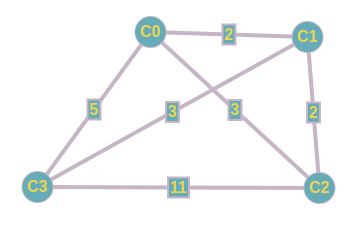
\includegraphics[width=9cm, height=6cm]{question3image} \\
1. In this graph, we begin at $C_0$. The shortest distance is $C_0 \rightarrow C_1$. Move to $C_1$ and mark $C_0$ as visited. \\
2. Then at $C_1$, the shortest distacne is $C_1 \rightarrow C_2$ without visited cities. Move to $C_2$ and mark $C_1$ as visited. \\
3. Then at $C_2$, the shortest distacne is $C_2 \rightarrow C_3$ without visited cities. Move to $C_3$ and mark $C_2$ as visited. \\
4. Then at $C_3$, the shortest distacne is $C_3 \rightarrow C_4$ without visited cities. Move to $C_4$ and mark $C_3$ as visited. \\
5. All cites visited and back to $C_0$. \par
The total distacne is $2+2+11+5 = 20$.
However, if we follow the path $C_0 \rightarrow C_2 \rightarrow C_1 \rightarrow C_3 \rightarrow C_0$, the total distance will be $3+2+3+5=13$.
Thus, my algorithm does works but does not find the correct answer. \\
\noindent \\
\textbf{running time:} \par
My algorithm visits all cities exactly once. Thus the time is $O(|V|)$, where $|V|$ means the number of all cities.


\pagebreak
\noindent
\large Question 4: \par
\normalsize 
\setlength{\baselineskip}{8mm}
Based on description of question, I think this procedure does not give me the correct shortest path from $s$ to $t$.
For example: \\
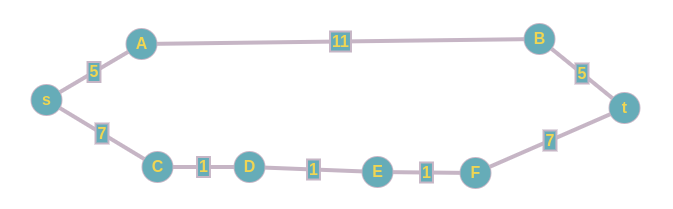
\includegraphics[width=12cm, height=4cm]{question4image} \par
In this example, we parallely use Dijkstra’s algorithm for node $t$ and node $s$. 
Since the length $l(s, A)$ is shorter than $l(s, C)$ and $l(t, B)$ is shorter than $l(t, F)$, the $dist(A)$ will be smaller than $dist(C)$ and $dist(B)$ will be smaller than $dist(B)$.
Then there will be a overlap between node $A$ and node $B$ without finding the real shortest path. 
Based on description, $d_1 = 5 + 11$, $d_2 = 5$, $d_1 + d_2 = 21$. This is incorrect. \par
Thus, this algorithm does not find the correct answer. \\


\pagebreak
\noindent
\large Question 5: \\
\normalsize 
\setlength{\baselineskip}{8mm}
\noindent
\textbf{(1):} \par
Based on description of question, I think the directed graph G seems as below. \\
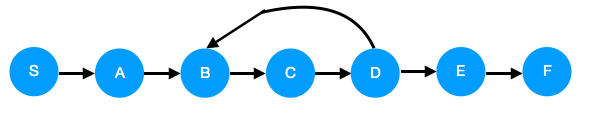
\includegraphics[width=14cm, height=3cm]{question5image} \par
The infinite path $p$ is infinite sequence $s, a, b, c, d, b, c ,d, b, c, ..., b, c, d, f$, where "..." is infinite. 
The $Inf(p)$ will be a set $\{b, c, d\}$. \\
\\
\textbf{Claim: } If $p$ is an infinite path of $G$, then the $Inf(p)$ is a subset of a single strongly connected component of $G$. \\
\textbf{Proof: } By contradiction. Suppose $p$ is an infinite path of $G$, and the $Inf(p)$ is not a subset of a single strongly connected component of $G$. 
Based on description and my example, the vertices in an infinite path $p$ are visited infinitely often because there is a cycle. 
The $Inf(p)$ is the set of vertices that occur infinitely many times in p. Therefore, the vertices in this set are connected by some directed path.
The defination of SCC is: in a directed graph, SCC is a set of nodes such that there is a (directed) path between every pair in both directions.
Based on defination of SCC, for each set of a single strongly connected component of $G$, their nodes are connected by a path. 
Since the vertices in $Inf(p)$ are all connected, the $Inf(p)$ must be a subset of a single strongly connected component of G. 
There is a contradiction and my suppose is incorrect. The claim holds.



\pagebreak
\noindent
\large Question 6: \\
\normalsize 
\setlength{\baselineskip}{8mm}
\noindent
\textbf{(2):} \par
If graph $G$ has an infinite path, then there will be a cycle in $G$.
Since $G$ has a finite number of vertices, only in a cycle, some vertices of $G$ are able to be visited infinitely often. \par
Thus, my algorithm is to determine if $G$ has a cycle.
I use DFS on $G$. If depth-first search reveals a back edge of a directed graph $G$, $G$ has a cycle and there is a infinite path. 
If we explore all nodes and there does not exist a back edge, then $G$ does not has an infinite path.   \\
\\
\textbf{Claim: } If the DFS reveals a back edge, the graph has a cycle.\\
\textbf{Proof: } let $(c, s)$ be a back edge from node $c$ to node $s$. By definition of back edge, $s$ is an ancestor of $c$.
In the DFS tree, there is a path from $s$ to $c$. The path $s \rightarrow c$ and back edge $(c, s)$ form a cycle. The claim holds. \\
\\
\textbf{running time:} \par
My algorithm is the same as basic DFS. Thus my running time is $O(|V| + |E|)$.



\pagebreak
\large \textbf{Extra}:\\ \vspace{5mm}\par
\normalsize 
\setlength{\baselineskip}{8mm}
My algorithm is using Breadth-first search. First find all cities which are reachable from City S by a cable which is less than L.
Then find all cities where are reachable from explored cities by cables which are less than L. 
Repeat this process untill find City T. \par
In this question, if the city is not reachable from City S by suitable cable, we will not visit them. We care about the length of cables. 
Therefore, the running time is $O(|E|)$.





\end{document} 







